\chapter{Implementation}
\label{cha:implementation}

\section{Core-Logic}
Blockchain-Identity is always focus around two actors: The user and his interaction with the blockchain and identity providers and their interaction with the user in an on- and off-blockchain fashion. We model our system in the same way but needed to make some specifications for the provider service which comes with two different motivations and rights:

\begin{itemize}
\item \textbf{Normal Provider}: Holds domain specific personal data about their consumers that are not exposed to the outside world. They have an interest in requesting user data to extend their system and to make new costumer registration easier. This services are untrusted and can not write to the blockchain. However they can read from the blockchain to verify transactions or extract information out of it. In general everyone can setup a provider service and request user data. They don’t need to be verified in any kind. 
\item \textbf{Government}: Single trusted entity that holds verifiable citizen information. This information are backed by the representative citizen office or other federal trusted institutions. The government usually verifies user data.
The government service is the only service that can read and write to the blockchain. 

The client application, on the other hand, has read and write rights and can interact with this providers.

This following sections descriptes the different provider/client applications and their interactions with the other components: frontend, Etherem-Blockchain-Adapter – EBA and the database.
\end{itemize}

\subsection{Motivation}
Since we are dealing with provider which are providing user information data we decided to implement a normal client-server architecture. Here we can use all the advantages TCP is providing us like transport layer encryption with SSL/TLS and the reliability/inorder-delivery TCP comes with. Where we would have to deal with our own encrypt-scheme if we would use UDP with peer-to-peer communication and port discovery, even if peer-to-peer communication seems like the more fitting solution since we are already in the domain of blockchain and decentralized applications. 

Choosing a client-server architecture comes with the drawback that the government service can not notify the client about incoming messages. The communication via the blockchain is not possible since the provider have not permission to write to it. To overcome this challenge we implemented a discovery service where each components registers to on bootstrap. (See section \ref{sec:discoveryService}).

We further decided to design our services RESTful (Representational state transfer). This in mind spring boot\footnote{\url{https://projects.spring.io/spring-boot/}} is a good choice in the Java domain for rapid prototyping. Spring boot also offers good integration for database adapters and spring security\footnote{\url{https://projects.spring.io/spring-security/}} a authentication and authorization framework. 

\subsubsection{Tools and Technologies}
Besides Sprint Boot and Spring Security we further committed us to the following technology stack: 

\begin{itemize}
\item Springfox\footnote{\url{https://springfox.github.io/springfox/}}: A API documentation framework. Additionally is is specifically designed for spring boot.
\item Feigen\footnote{\url{https://github.com/OpenFeign/feign}}: Framework that make writing API calls easier. You only need to provide an interface and specify it with annotations to produce a HTTP request to specific domain. Mapping and error handling is mostly done by Feigen. 
\item Lombok\footnote{\url{https://projectlombok.org/}}: Lombok reduces the boilerplate code in Java by directly translating data or logging annotation into java byte code. It helps us to reduce the size of our models to a minimum by obscuring the setter, getter and constructors. 
\item Bouncy Castle\footnote{\url{https://www.bouncycastle.org/java.html}}: The unofficial default cryptographic library for java. It implements the java security provider interface and provides a functions like RSA encryption or signature mechanism.
\item Zxing\footnote{\url{https://github.com/zxing/zxing}}: Library to generate QR- and bar-codes. 
\item Web3j\footnote{\url{https://web3j.io/}}: Library providing the Ethereum adapter. (More in section \ref{section:eba}. In this section this library is mainly used to generate ECDSA (Elliptic Curve with Digital Signature Algorithm) signatures. 
\end{itemize}

Further the following technologies are used for testing:

\begin{itemize}
\item AssertJ\footnote{\url{https://joel-costigliola.github.io/assertj/}}: A fluent assertion semantic for java. 
\item Mockito\footnote{\url{http://site.mockito.org/}}: Mocking library to make unit and rest test more modular and encapsulated from outstanding components. 
\end{itemize}

\subsection{Claims}
The Blockchain-Identity is centralized around user claims. Claims are bits of personal information, that can be made about a person. It shell describe the an atomic unit of information you receive if you continue to cut bigger personal information chunks into smaller onces. We introduce 5 different claim types: 

\begin{itemize}
\item \textbf{Boolean}: Boolean-claims are claims that can be answered with a simple yes or no answer.
Example: "Has HVI?" 
\item \textbf{String}: String-claims are the most common onces. They shell not be longer then one word or name. 
Example: "Which street lives Bob in?"
\item \textbf{Number}: Number-claims hold numbers (in double representation) as values. 
Example: "What is Bobs ZIP code?"
\item \textbf{Date}: Date-claims relate to claims that referee to a specific time or date. They are saved as LocalDateTime objects.
Example: "When was Bob born?"  
\item \textbf{Object}: All other claims that are not representable with the above definitions needs to be saved as generic objects. This may be lists of claims, or even more complex representations like whole documents. Since we decided that in our prototype you can break down every claim in a subset of the above definition, this claim is lacking support in a closure related context. 
Example: "What is Bobs whole medical record?"
\end{itemize}

The claim are structured all over the system in the save way. In their core they consist of ID, type and value. The ID defines a unique string that is well defined and is strictly bound to a claim type. 
An overview about all current defined claim IDs can be found in appendix \ref{appendix:claimID}. Claim IDs are explicitly choose as strings and not an enums since they shell be expendable and each provider shell be able to include their own claim IDs if they are not yet present. If an wrong type is defined for a claim an exception will raise. 

The claim type is bound to claim operations. Claim operations are logical operations that can be interpreted by the closure expression engine. We will introduce in detail how that work in section \ref{sec:closure}. 

The claim value is simply from type object. Some could had imagine that it shell be a generic, but they are hard to serialize and deserialize. Since generic’s type are defined on compile time and claims are often read from and to the database and send via the network, the overhead of type determination would be larger then just parsing it into an object and checking the type manual. 

Claims also hold some meta information about who is the issuer (reference to the provider, original issuing this claim), and a modification date which gets updated each time a claim is changed. The modification date enables us to see if a claim is outdated and needs to be updated again. Claims are of nature unsigned, but can be signed by on request. 

\subsection{Components}
\begin{figure}
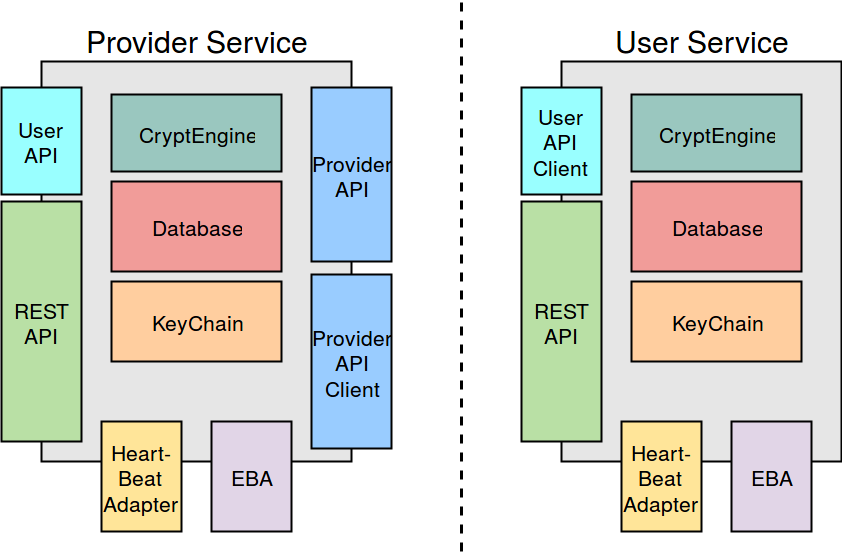
\includegraphics[width=0.7\textwidth]{impl/ComponentDiagram.png}
\centering
\caption{Overview about the components of an individual service and their exposed endpoints. Left is the provider service providing also a provider API and provider API client. Right the user service implementing the client API client.}
\label{fig:componentDiagram}
\end{figure}

In figure \ref{fig:componentDiagram} you can see an overview about the components in the provider and user service. All boxes that are drown over the border are representations of exposed endpoints or clients and inside the box are the core components listed.

\subsubsection{Internal components}
The crypt engine is the main framework for encrypting, decrypting, signing, validating signatures and generating hashes. It provides methods for symmetric and asymmetric encryption. It uses bouncy castles as security provider to generate keys and handle cryptography. To generate elliptic curve signatures it uses the framework provided by web3j. 

We are using spring data to provide a very easy interface to couchbase, our database storage (section \ref{sec:database}). The keychain is the current session object holding the RSA key-pair, EC key-pair and some other meta information about the current state of the service. This objects gets cleared if the services logs out and restored if the service logs in (section \ref{sec:registerContract}). 

\subsubsection{User API}
\label{sec:userAPI}
The user api provided by a provider service and requested by the user service defines the central entry point of client requests to a provider. The user and the provider API (section \ref{sec:providerAPI} is implemented as a normal Java interface. The provider service is implementing this interface and mapping the defined methods to REST endpoints which then are bounded to a predefined paths. The user service on the other hand, extends this interface in a new interface which then serves as a Feign adapter bound to the same predefined paths. This is really convenient because Feign needs an annotated interface to build an REST client out if it. We only have to bind Feign to the same resources paths the provider is exposing so that they can communicate to each other. 

\subsubsection{Provider API}
\label{sec:providerAPI}
The provider API is a unified interface which each provider is offering in form of REST endpoints. Each provider builds also a Feign client (see section \ref{sec:userAPI}) to talk to other providers.  Via this API provider an interact with each other to exchange requests or offering services. Notably is that each request needs to be authenticated via a SignedRequest (see section \ref{sec:ecdsa}) to ensure that only authenticated entities request this API. 

\subsubsection{REST API}
The rest API is the connection to the frontend. Here the frontend can ask for user resources and claims to display them a web admin or the end user. This requests are backed by a basic authentication mechanism which is not optimal because the password and user name is transmitted in plain text if no transport layer encryption is used. The plan was to change this mechanism since to a more secure scheme like Json-Web-Token (JWT) authentication, but that would require changes in other components and was also out of scope of the core focus of this project. 

\subsubsection{HeartBeatAdapter and EBA}
Ethereum Blockchain Adapter (EBA) is the entry point to communicate with the blockchain. We defined an interface (EBAInterface) between the blockchain component and the core-logic to develop in a parallel fashion. Relate to the section \ref{sec:eba} where everything related to the blockchain is explained.

The HeartBeatAdapter is the connection to the Discovery Service (section \ref{sec:discoveryService}). A service can register itself to the discovery service, create or subscribe to new beats.

\subsection{Notable methods}
The follow sections describe problem and challenges that occurred during development.

\subsubsection{Serializing and deserialization of arbitrary objects}
\label{sec:serialobject}

Serialization of arbitrary objects is a challenge in systems where the order of serialization is imported (e.g. building a signature via hashing over the serialization outcome). A common serialization method is the JSON-String serialization, where an arbitrary object state gets converted into a JSON representation. This can be done by (for example) the Jackson object mapper\footnote{\url{https://github.com/FasterXML/jackson}}. We need, however, define the order  in which each field of the object gets serialized. Serializing all objects into JSON representation allows us to serialize the objects in the same way all the time, no matter if it is a signed request against the blockchain or a response to the frontend. 

The other approach is to use Javas serialization API. Classes that implement "Serializable" will then be converted to a stream which then can be collected to a byte array. Since Java serialization will take care of the serialization order by itself we don’t have to bother with that. 

However, we need to find a unique way to serialize objects since building a hash-based signature via objects must be done always in the same way, no matter on which system the signing or verification of the signature is happening. We decided to use JSON serialization approach (with explicitly defining the order in which properties shell be serialized) since it is language independent, easier to implement and to debug, even if it is not as efficient as raw byte representation. How signatures are build and verified is described in the next section \ref{sec:ecdsa}. 

The implementation of sets in the Java Virtual Machine needed also consideration. Sets are of nature unordered and it depends on the order of object initialization on the heap to define the real order the elements returned in. If you want the same order of object each time, you need to use lists. Building a hash over an object holding sets is obviously a bad idea since the order of attributes may be different from machine to machine, so the hash will be a different.  

Another problem related to serialization was that variables of type "Object" will be converted into a string representation and on deseralization this string will not be converted back in the original type since "String" itself extends "Object". This became a problem on serialization of LocalDateTime values, which were not parsed back into a LocalDateTime. 

To temporary handle the different conversions we implemented a "ValueHolder", a simple class separating LocalDateTime values from generic Object values. By converting explicit into a LocalDateTime the Jackson converter recognizes the string representation and deserialize it into the correct object representation. Future improvements can be made by including the target class of the serialized value as meta information, so that in deseralization the value can be parsed back to its original class. Further the object mapper need to be adapted adequately. 

\subsubsection{ECDSA and SignedRequests}
\label{sec:ecdsa}

Elliptic Curve Digital Signature Algorithm (ECDSA) in the SECP256k1 configuration is used by Bitcoin and Ethereum to sign transaction to the blockchain. \cite{mayer2016ecdsa} This ensures integrity and authenticity to the sender and the content of the transaction. 

To populate this security properties also between services we use ECDSA also for inter service communication. This is done by generating a so called "signedRequest". This object can hold a generic payload and the EC Digital-Signature over this payload. This payload but needs to include the ethereum address of the sender (similar to ethereum transactions). A signature is then build in the following way: 

\begin{enumerate}
\item The payload (holding also the ethereum address of the signer) gets converted to a JSON as defined in section \ref{sec:serialobject}
\item A SHA-256 hash is build over the given JSON
\item This hash will then be signed by the ECDSA and the private key (EC) of the signer
\item The resulting signature gets appended in the signed request for validation
\end{enumerate}

\noindent The validator on the other hand can validate the signature by applying the following steps:

\begin{enumerate}
\item Convert the payload to a JSON with the same object mapper configuration as used for serialization.
\item Create a SHA-256 hash itself over the generated JSON
\item Validate the provided signature against the computed hash. Interesting to know is that his validation does not yield a boolean flag but a computed ethereum address the algorithm "thinks" that signed the request. 
\item We take this generated ethereum address to check it against the included ethereum address in the payload. If they are equal yield true, else false. 
\end{enumerate}

If we would not have include the ethereum address of the sender inside the signed payload an malicious attacker may have exchanged it against a valid signature address. 
To validate and build signatures over Java objects we are using the Jackson object mapper module \lstinline{jackson-datatype-jsr310} in version \lstinline{2.8.10}. This module is further configuration to write time values as a time stamp in the ISO-8601 format. 

\subsection{Discovery Service}
\label{sec:discoveryService}
As mentioned in the previous section the Discovery Service is the result of a client-server architecture in a peer-to-peer environment. But it further serves additional purpose for holding and distributing RSA public keys, discovering domain names, where to find the exposed API and if the requested service is online. 

While all the stored information is public visible no sensitive data is exposed in the Discovery Service. It just provides connection information and serves as a message broker. Each stored entry needs to be signed by the author with the private key bound to his ethereum address. All unauthorized requests are rejected by the service. By ensuring the authenticity of each entry creation or update it is ensured that no service spoofing can happen. Only the holder of the private key bound to his ethereum address can update his connection information.

\subsubsection{Beats}
\label{sec:beats}
Beats are the messages that are routed by the Discovery Service. A \textit{beat} a small package containing an event type describing that kind of message it is and a subject field referencing the location where the new information is to find. Each beat is uniquely identified by the combination of recipient ethereum address and the current beat number (incrementing per beat). 

There are two types of subjects: The URL references a API endpoint where new or updates information are now present. The recipient is requested to request this API endpoint to update his information state. The other kind of subject is a ethereum address: The recipient is requested to query the blockchain for the given address to process the information stored at this address. 

On registration entities start to periodically (each 10 seconds) ping the Discovery Service to wait for new incoming beats. Since the discovery service itself is not a trusted entity, each beat gets verified before processing and it is checked that the signature matches the senders ethereum address.

\subsubsection{PKI}
\label{sec:pki}

A Public-Key-Infrastructure (PKI) is an infrastructure to bound identities to public keys. This usually relay on trust in either a Certificate Authority or on other users trusting this public key. 

Since each entity stores also his RSA public key into the discovery service and sign this entry with his EC private key, the trust of the given RSA public key is tightly bound this EC key pair. If the RSA key gets stolen it can be simply replaced in the Discovery Service. If the EC key gets stolen both key pairs need to be regenerated. How we establish trust in the EC key pair is explained in the next section.

\subsection{Registration}
\label{sec:registerContract}
\begin{figure}
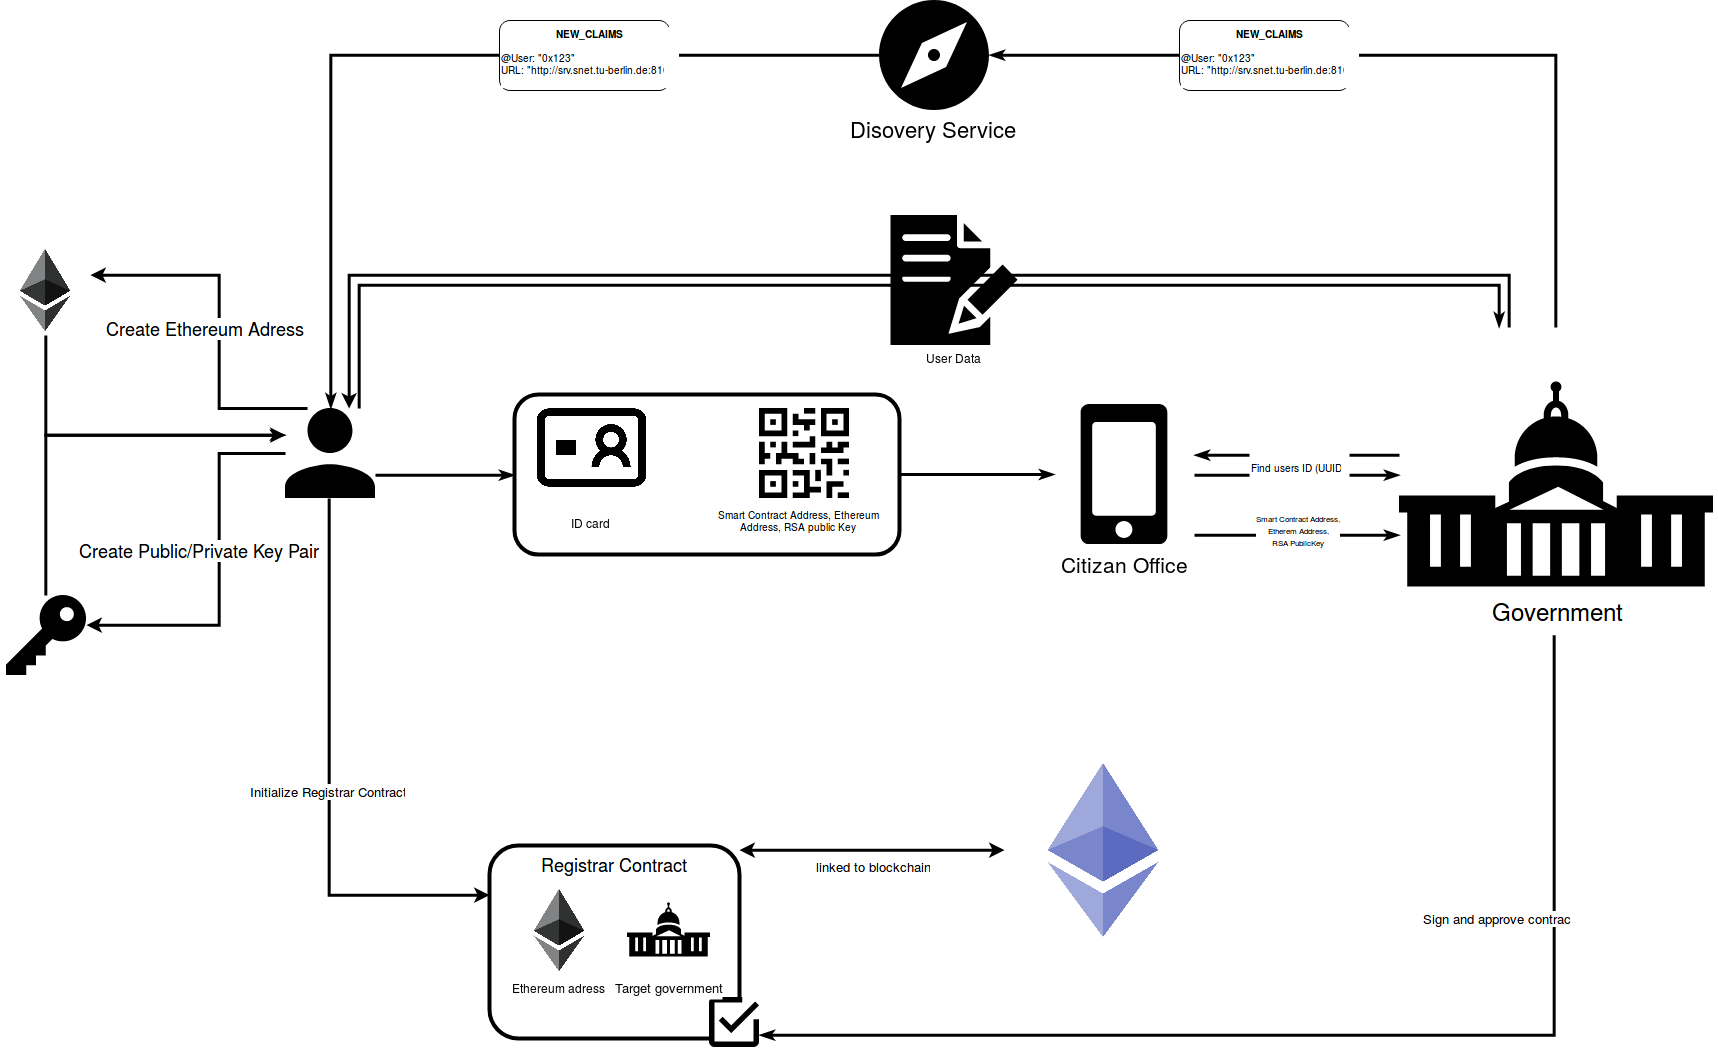
\includegraphics[width=\textwidth]{impl/RegisterContractImpl.png}
\centering
\caption{Implementation of the Register Contract flow. Since it was not possible (time limitations) to include the eID verification mechanism, we implemented the in-person verification. Here the newly register user has to go the citizen office to how his ID card to gets his ethereum address, RSA public key and smart contract address verified.}
\label{fig:registerContractImpl}
\end{figure}

To start the register process the user services exposes the unsecured resources "Account" which provides action endpoints for login, logout, register and QR-code retrieval (later more on that), where the web client can make a HTTP-POST call to "account/register" with a newly set password.
This call will trigger three main actions:

\begin{enumerate}
\item Creating a 4096-bit security RSA key pair
\item Creating a new wallet containing EC-Key Pair 
\item Setting up the register contract 
\end{enumerate}

\subsubsection{Creating RSA and EC key pairs}
We need the RSA key-pair to later encrypt sensitive data that is send via the blockchain since the blockchain itself is a public ledger and for everyone readable. The key-pair created by web3j does not provide any confidentiality since the ECDSA (Elliptic Curve Digital Signature Algorithm) can only be used to generate and verify signatures (see section \ref{sec:ecdsa}). So the users creates a 4096-bit strong RSA key pair (step 1.1). So ensure that this key indeed belongs to the newly generated EC key-pair (step 1.2) we generate a signature, as mentioned previously (section \ref{sec:pki}), over the RSA public key with the EC private key and publish this information to the discovery service.

We further also save our keys, password based symmetric encrypted, to our data directory under \lstinline|{$USER.HOME}./ethereum/blockchain-identity/|\footnote{The "./ethereum" directory is the default directory to save all ethereum related files.}. If the user later logs out, we can simply remove the current RSA and EC keys from memory and if the user logs in again, providing his password, we can decrypt the wallet files and read the RSA and EC keys back in memory. 

The user service application is planned to run locally on the users host machine. This would secure it from outside access. Since we, because of time limitations, didn’t manage to implement a key recovery mechanism there might be an Denial-of-Service attack vector possible where a malicious application running also locally on the users host machine, call periodically the register-endpoint, preventing the user from accessing his information because his keys gets reshuffled every time. Some could think about disabling this register endpoint after successful creating a key pair, but since this is a prototype under developing this endpoint needs to be open and accessible. 

\subsubsection{Deploying the register contract}
The ethereum address itself is a just a representation of the EC public key. To now register the user that is bound to his ethereum address we setup a register contract (step 2.). This register contract is just a public representation of the unverified user and contains no more information then the users ethereum address and a flag if the user is approved. This flag can only be set by the trusted government. 

\subsubsection{Verifying the user}
As shown in figure \ref{fig:registerContractImpl} the user then creates a QR-Code (step 3.) to encode his ethereum address, address of the smart contract and his public key into it.\footnote{It is not necessary to encode the public key into the QR-code at all since the Discovery Service also stores this information, but we can save an additional request from the government side to discover it by providing it in the register flow directly.} The QR-code generation is done with the help of the Xzing library and exposed via an rest endpoint "/account/qr-code". The idea to generate a QR-code is simply that ethereum addresses are quite hard to type and since the user has to go to the citizen office in person he might as well just show is representative QR-code. 

The citizen office verifies that the user is indeed who he claims to be with the use of the provided ID card. The android application build for the purpose of scanning the QR-code, generating a signature over the retrieved information and sending it to the government service, needs further know which user is currently trying to be verified to the system. To do so the citizen office types in the user information found on the ID card, for example given name, family name, etc. to then send a authorized requests to the government which then queries its database for a user with the same information and returns his UUID (step 4.). 

With the retrieved UUID the application can then make a signed POST request to the user resource that tries to get verified and updates the user for his public key, ethereum address and register contract address (step 5.).

\subsubsection{Finalize user registration}
The government then uses the information about the user to update the register contract to set the approval flag to true (step 6.). So that every party in the system observing the blockchain can verify that the user holding the private key for the ethereum address is indeed verified by the government. If each provider checks that he is only communicating with verified users we are preventing sibyl attacks in the most effective way possible. There would be no need to use CAPTURES since only verified users are able to interact with the system. 

It also creates a new signed beat (section \ref{sec:beats}, step 7.1 and 7.2) with the information "NEW\_CLAIMS" addressed at the users ethereum address to notify the user to request its provider API (section \ref{sec:providerAPI} to retrieve the claims stored at the government about him (step 8.). 

Since a new user is now verified in the system other provider shell also send the user their claims about him. That point was really difficult to implement and was left open for further work since there are open unanswered questions: How do provider assign the new ethereum address of the newly registered user to any user of their system (you can not broadcast any user claims over the network because of privacy reasons)? How to ensure that provider send all their claims (since they are not trusted they might be malicious)? 
In the end we said that the user has to manually notify provider about his presents in the system.

\subsection{Permission Requests}
\label{sec:ppr}

\begin{figure}
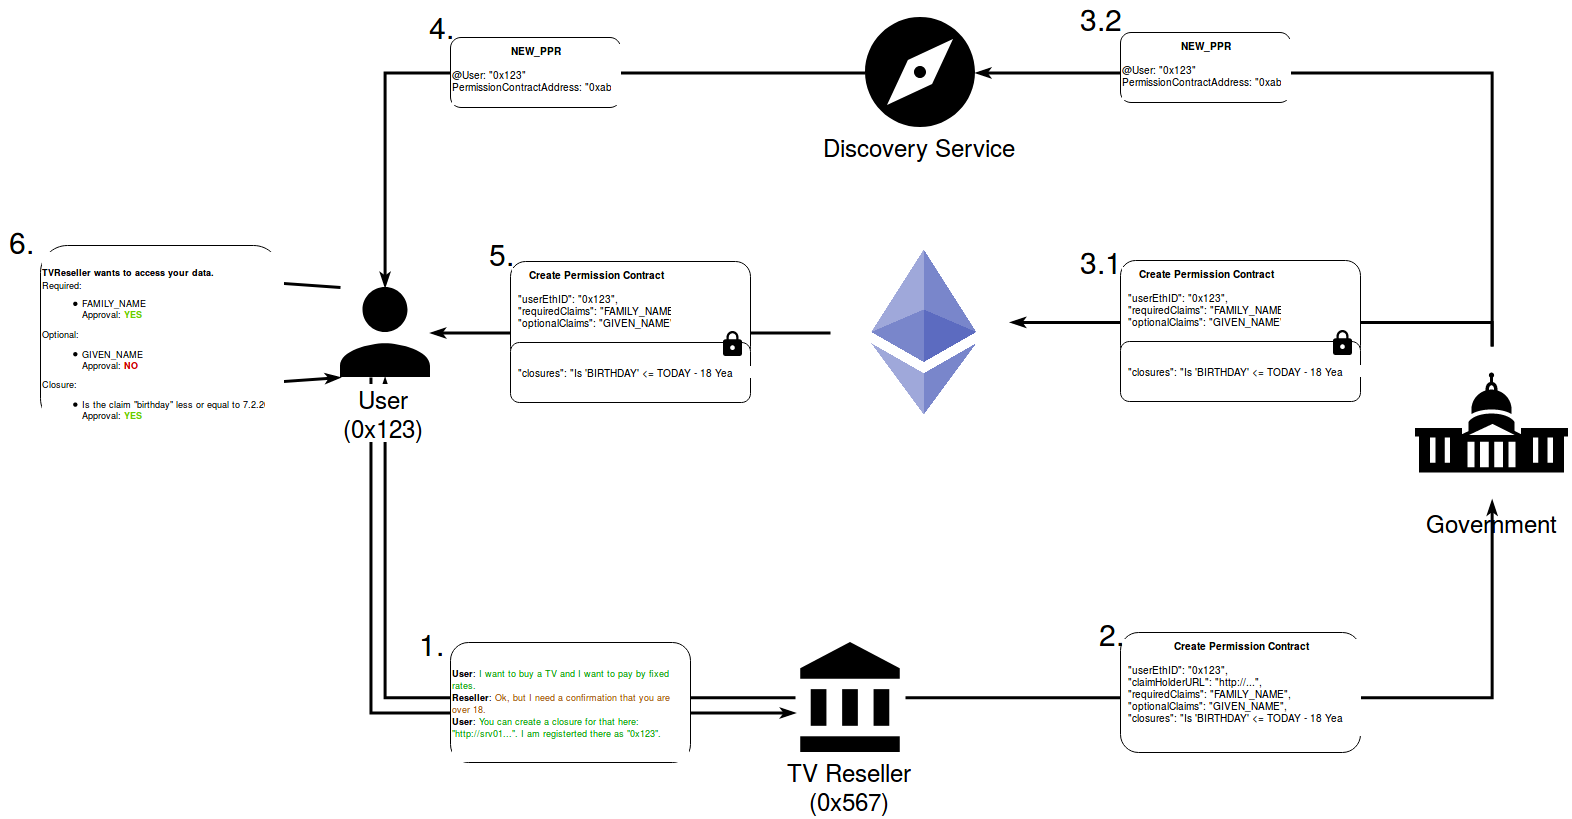
\includegraphics[width=\textwidth]{impl/PPR_closure_1.png}
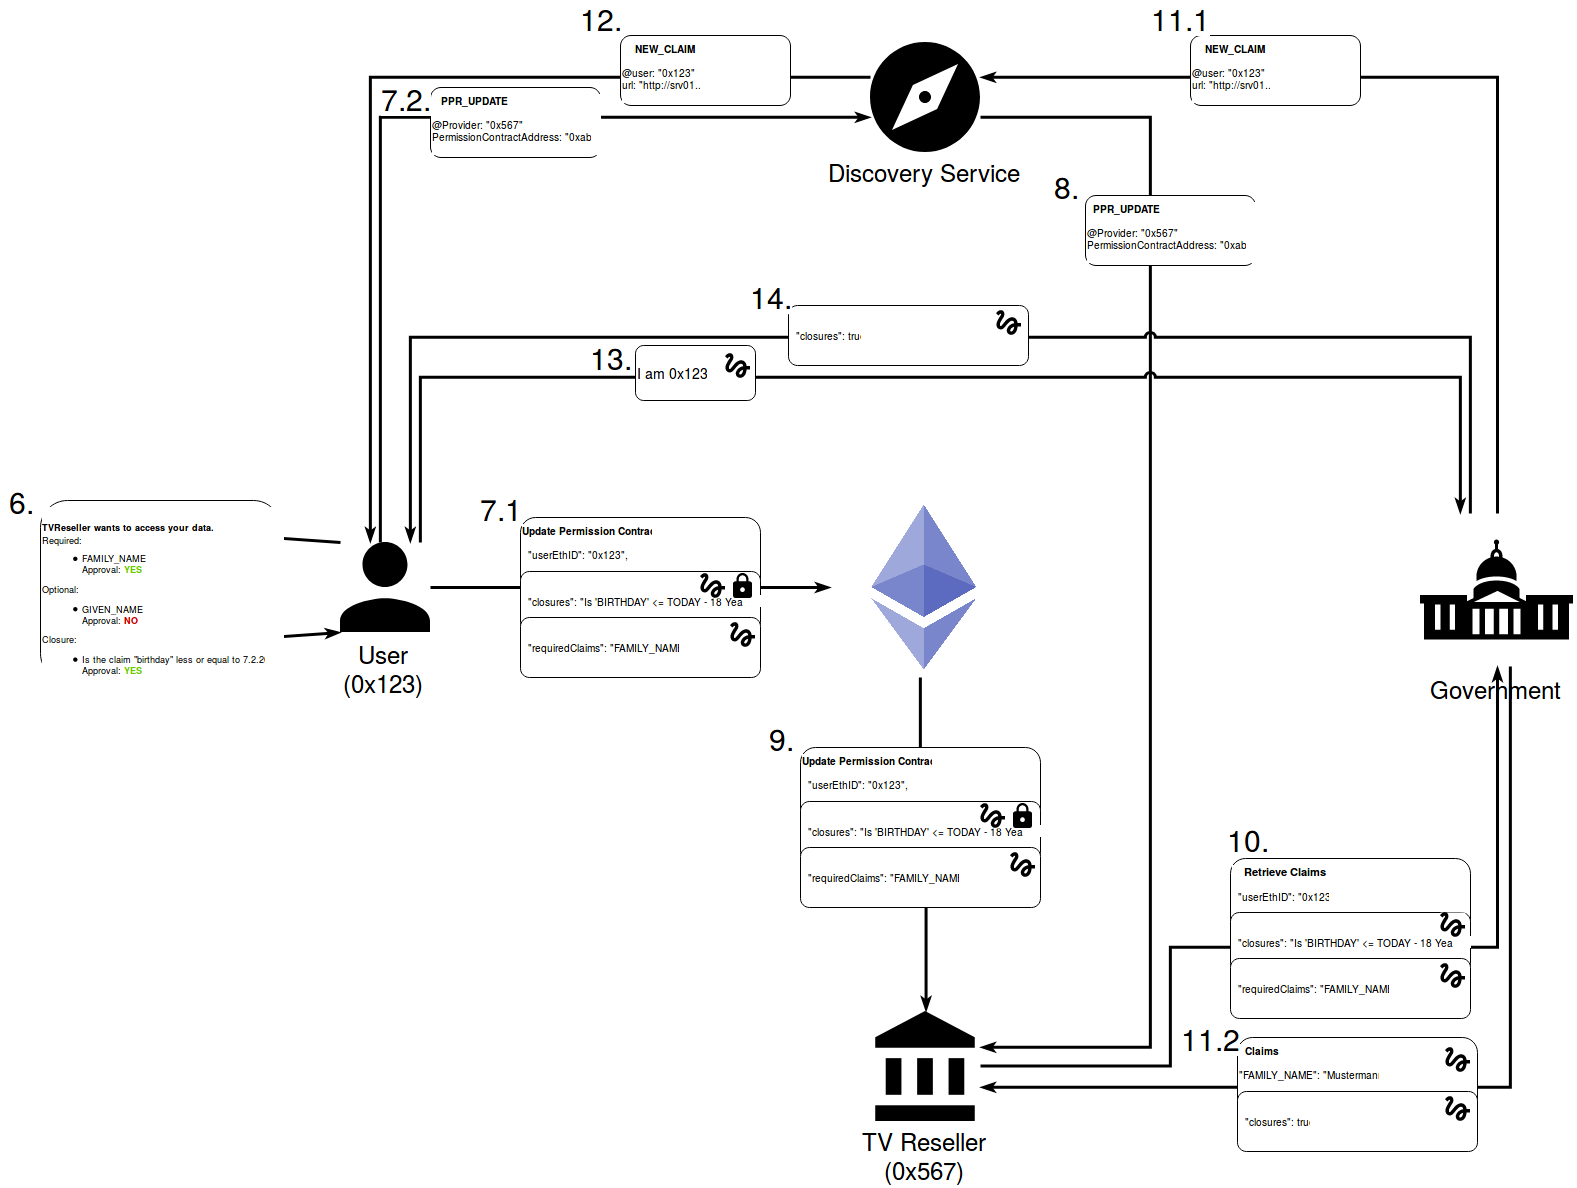
\includegraphics[width=\textwidth]{impl/PPR_closure_2.png}
\centering
\caption{Flow to request permission about GIVEN\_NAME (optional) and FAMILY\_NAME (required) and a closure over the age of the user.}
\label{fig:ppr}
\end{figure}

Located in the core of our project stand the Provider Permission Request (PPR). Its goal is to ensure that every request about personal information es routed to the user, which can approve or disapprove the information population. With PPR-Contracts it is further possible to see which provider holds which data about which (pseudonymous) user. To implement a the PPR flow we need all of the previous introduced technologies since all service need to play together to implement the PPR. 

We start by the provider requesting the user information (step 2.). Please ignore the closure reference in the figure \ref{fig:ppr} they will be explained separately.  The frontend receiving the users ethereum address, that was populated to the network in the register contract (section \ref{sec:registerContract}), and a URL referencing the provider holding the claims that shell be shared (step 1.). The last bit of information are the claim IDs that shell be requested. The application differences between required and optional claims \ref{sec:claims}. Required claims needs either approval by the user or the whole PPR will be discard. Optional claims can be partially accepted or rejected by the user, the PPR will still be executed. So the provider sets the claim IDs appropriately and signs this PPR objects and sends it to the provider holding the claims about the requested user. In return he will retrieve the smart contract address of the created PPR contract. He creates also a PPR meta object that holds the current state of the pending PPR and saves this object in his database. 

The information what claims are are known about a user of a provider is exposed through an unsecured endpoint. This endpoint is not providing the values to the claims, rather it only exposes the claim IDs, types and operations. We consider this information not critical to protect, since this are the same information anyone can read from the blockchain. Further work can think about a mechanism to protect this information since they might enable attackers to locate valuable targets. 

This provider is in our case the government service and so a trusted service that can also write to the blockchain. Please note that we can create PPRs to every provider that is able to write to the blockchain. We government service will proceed to process the request, by first verifying the signature and second checking if the requested claims match the claims the targeted user hold. 

In Step 3.1 the government is populating the received information in form of a smart contract to the blockchain. This smart contract is addressed to the user that is the owner of the requested claims. Parallel in step 3.2. the user is notified via a new beat referencing the current created smart contract.
This beat gets read by the user in step 4. and processed by retrieving the smart contract from the blockchain in step 5. Since all information about the claims in PPR are unencrypted everyone can ensure that a PPR was created over the defined claims IDs and that the user is now processing the PPR. He is doing so by saving the PPR in his database and creating a new message to notify the frontend that a new PPR was retrieved. In Step 6 the frontend now asks the user for his explicit approval. As mentioned previous a rejection of all required claims would result in a rejection of the PPR itself. It would still be updated in the blockchain so that the requesting provider know that the PPR was rejected. To approve the PPR the user must accept the sharing of all required claims and can decide which optional claims he wants to share.  

Upon receiving the information which claims the user approved, the user service generates a signature over the claim IDs that were approved. This is done in the form of a signed request over the claim ID. We need also to include the providers address in to the signature to ensure that the signed request gets not reused by other provider. Finally object mapper is used to translate this object into a JSON string (later needed to send this JSON to the government) and then converting this string into base64 representation (get rid of any non ASCII characters to ensure compatibility with the ethereum seralization) to put it into the blockchain (step 7.1). Unapproved requests will not receive a signature. We are not encrypting this signature in anyway since everybody shell take note that the user approved the PPR entry. This will ensure that the user can not later deny to has approved this PPR entry. To also notify the requesting provider that the user updated the PPR contract, the user service is creating a new beat addressed at the provider that initially requested the claims, referencing the updated permission contract (step 7.2). 

The provider registers this beat (step 8.) and can now pull the updated PPR information from the blockchain. He evaluates whether the contract was at all approved (if all required claims were signed) and updates the PPR meta object in his database with the information about approved claims. This object can later be used to display administrator which claims get usually approved and serves further as a permission history for each user. 

To finally retrieve the claim values in step 11.2 the provider uses the by the user signed JSON strings to query the government service for the claim values. The government service on the other hand can verify the signature of the user and so knows that the user explicitly approved to share the given claims. He also verifies that the requesting provider is indeed the provider the user granted permission (remember that the provider address is also signed by the user). If all requirements are fulfilled the claims matching the claim IDs in the requests are returned (step 11.2).

Here ends the permission request. The following steps are only an extension to handle closure requests accordingly. They will be described in the next section.     

\subsection{Closures}
\label{sec:closure}
Closures are boolean expressions that do not reveal information about the actual claim value. For example is a common closure “Is Bob over 18?”. We can answer this question with yes or no but we do not reveal Bobs birthday. However we see the question as a semi critical personal information which needs to be protected. Semi since it is not a essential personal information and it is not fatal if the encryption got broken in the future and we can not remove the closure from the blockchain. However, we encrypt the compared value, so that some only see the closure “Is Bob over XXX?”. In this case it might be easy to guess, but the point is that closures in general remain public visible, while the compared value remains secret. So everybody can still see that an exchange happened, but does can not gain any new information about Bob. 

The closure flow is tightly bound to the permission request flow. They both are displayed in the figure \ref{fig:ppr}.  We start off by step 1. where the TV reseller want a closure over the users age and wants to know if the user is over 18 years old. As already known from the PPR flow the provider does now request the government service for the respective closure. 

A closure in code form consist of three values: 

\begin{itemize}
\item \textbf{claim ID}: References the claim that shell be used for the closure evaluation. 
\item \textbf{claim operation}: Defines a logical operation that shell be used as comparator. 
\item \textbf{static value}: The value which shell be used for comparison. 
\end{itemize}

The type of the requested claim defines which operations are supported (appendix \ref{appendix:claimOperation} and sets the type that the static value needs to have. Indeed it makes no sense to compare a string to a number. Claims from type objects are not yet supported for closures since it is not easy to find a unique set of operations that are executable of them. We thought about using a JSON query language that let us query arbitrary JSON objects and compare their properties to other values. First this seemed like a good and powerful solution but later it was clear that is not piratical since the user needs to understand the expressions to either approve or reject them. We have no chance to parse the JSON query language to a user friendly representation. Also this query language would introduce new attack vectors at user claims and may also trick the user to approve a query that may select something complete different then the user though he would approved. Defining a static set of operations in such a inflexible fashion as we did, allowed us to parse a user friendly question out of it, so that every user understands what is requested. Further we also have the power to limit the expression language in that kind that no new attack vectors are introduced and expressions will not have any side effects. 

The government, as holder of the claim value, can verify that the claim operation and static value matches the type of the requested claim target. If all checks succeeded it will encrypt the static value using a newly generated symmetric session key (AES, 256 bit). To do so the static value will be converted into a byte representation and then encrypted. To now send the session key securely over to the user it is encrypted asymmetrically with the public key of the user (RSA, 4096 bit). We archive forward secrecy here since we it is a one time session key that is discarded after usage. Our closure is now secured and ready to be put into the blockchain in step 3.1. 

In step 5 the user extracts the closure from the blockchain by first decrypting the session key with his RSA private key. He now can decrypt the static values of the closure requests. After that is done we can request the claim values from the database of the user to evaluate the closure expression. This is done by simply evaluating the claim value with the given claim operation and the given static value. We further can now compute the user friendly description of the closure expression. Since we assigned each claim operation a lingual expression (see appendix \ref{appendix:claimOperation}), we have all components together to build up a question. To know if a person is over 18 years old an description of that in figure \ref{fig:closureDescribtion} is generated.

\begin{figure}
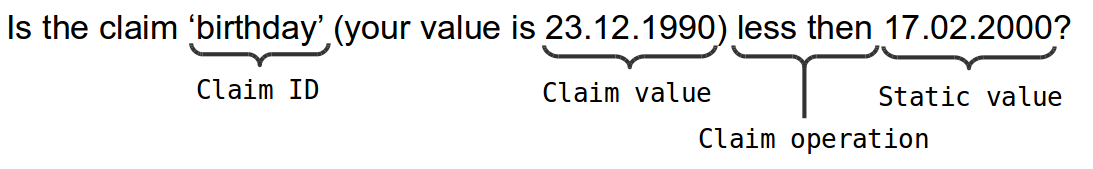
\includegraphics[width=0.6\textwidth]{impl/closure_describtion.png}
\centering
\caption{Components of a closure description that is generated to create a user friendly literal expression.}
\label{fig:closureDescribtion}
\end{figure}

The user can now decide to either approve or reject this closure. For each approved closure the closure is signed and the static value is again encrypted with a newly generated session key which is then again asymmetrically encrypted. The difference now is that the contract is now addressed to the requesting provider, so the static values need to be encrypted with the public key of the requesting provider. Since the user may not know this public key he can discover it. This is simply done by querying the discovery service that is holding all public keys to ethereum address mappings. The PPR is updated with the new information (step 7.1) and a new beat is created to notify the provider (step 7.2). 
